%%%%%%%%%%%%%%%%%%%%%%%%%%%%%%%%%%%%%%%%%%%%%%%%%%%%%%%%%%%%%%%%%%%%%%%%%%%%%%%
% Model Staruszkiewicza
%%%%%%%%%%%%%%%%%%%%%%%%%%%%%%%%%%%%%%%%%%%%%%%%%%%%%%%%%%%%%%%%%%%%%%%%%%%%%%%
\subsection{Fundametalny relatywistyczny rotator}
Przez nierelatywistyczny rotator rozumiemy układ dwóch mas punktowych
$m_1,\ m_2$ połączonych nieważkim
prętem długości $\ell$ (rys. \ref{classic_rotator}). Lagrangian 
takiego układu w układzie środka masy ma postać~\cite{landau1978krotki}
\begin{align}
L = \frac{m }{2} \left(\frac{\d r}{\d t}\right)^2, \quad m=m_1+m_2, r=r_2-r_1
\end{align}
gdzie $r_1,\ r_2$ to odpowiednio położenia mas $m_1$, $m_2$.
Zauważmy, że $||r|| =\ell = const$, a zatem interesuje nas jedynie kierunek 
wyznaczony przez $r$.
Wersor $ \hat{r} = r / \ell$ możemy przedstawić za pomocą  
współrzędnych sferycznych
\begin{align}
\hat{r} = ( \cos \phi \sin\theta, \ \sin\phi\sin\theta,\ \cos\theta )
\end{align}
Obracamy układ odniesienia tak, aby $\theta = \pi/2$. Lagrangian 
przyjmuje wtedy postać
\begin{align}
L = \frac{m\ell^2 }{2} \left(\frac{\d \phi}{\d t}\right)^2
\end{align}
Z równania Eulera-Lagranga dla $\phi$ wynika, że 
\begin{align}
\ddot{\phi} = 0
\end{align}
A zatem $\phi \sim t$, to znaczy, że 
nierelatywistyczny rotator mierzy Newtonowski czas
absolutny $t$. Skłania nas to do refleksji nad możliwością 
wykorzystania relatywistycznego rotatora 
do pomiarów czasu. Prostota układu sugeruje, że 
może on być odpowiedni do testowania hipotezy zegara.
\begin{figure}
\centering
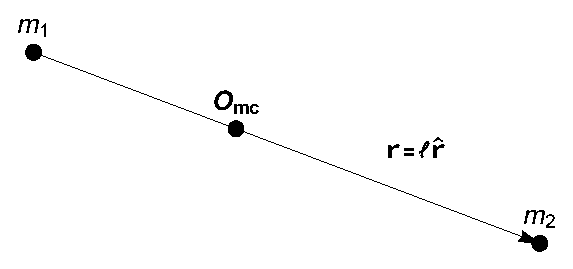
\includegraphics[scale=0.6]{classic_rotator2.eps}
\caption{Klasyczny rotator składający się z dwóch mas $m_1$, $m_2$ 
połączonych nieważkim prętem długości $\ell$.}
\label{classic_rotator}
\end{figure}

Przeniesienie układu na grunt relatywistyczny wprowadził 
profesor Staruszkiewicz~\cite{star2008} proponując następujące 
definicje:
\begin{definition}
Relatywistyczny rotator to układ dynamiczny
 opisany przez położenie $x$ i kierunek
zerowy $k$ oraz dodatkowo dwa parametry: masę $m$ i długość $\ell$.
\end{definition}
\begin{definition}
Układ dynamiczny  nazywamy fenomenologicznym jeżeli jego niezmienniki Casimira są 
całkami ruchu. Układ dynamiczny nazywamy fundamentalnym jeżeli jego niezmienniki
Casimira są parametrami - nie zależą od wartości początkowych.
\end{definition}
W oparciu o powyższe definicje można skonstruować fundamentalny
relatywistyczny rotator. Z wielkości zawartych w definicji relatywistycznego 
rotatora możemy utworzyć bezwymiarową wielkość
\begin{align}
\xi = - \ell^2 \frac{\dot{k} \cdot \dot{k}}{ ( k \cdot \dot{x})^2 }.
\end{align}
Możemy wtedy utworzyć Lagrangian postaci
\begin{align}
L = m \sqrt{ \dot{x} \cdot \dot{x} } f( \xi ) .
\end{align}
Działanie związane z powyższym Lagrangianem 
jest niezmiennicze ze względu reparametryzację, 
Lorenzowsko niezmiennicze. Dodatkowo $k$ wzkazuje kierunek zerowy, a zatem
 układ fizyczny nie wmienia się
po przeskalowaniu $k \to a k$. 
....

Niezmiennikami Casimira będą w tym przypadku $P_\mu P^\mu$ oraz
$W_\mu W^\mu$ gdzie 
\begin{align}
W_\mu = - \frac{1}{2} \varepsilon_{\mu\nu\rho\sigma}
M^{\nu\rho} P^\sigma
\end{align}


